\chapter{Server application}
\section{Application organization}
The server application has been developed and organized according to the multi-tier application paradigm.
\begin{figure}[!htb]
   \centering
   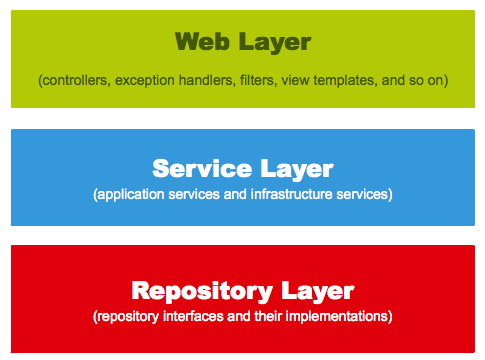
\includegraphics[width=.8\textwidth]{application_layers.png}
   \caption{Subdivision of layers of multi-tier application.}\label{Fig:AppMultiTier}
\end{figure}
Such paradigm is shown in figure \ref{Fig:AppMultiTier} and it states that a web application has to be subdivided in different layers, each one of them with its own responsabilities. It's an approach not so far from the \textit{divide et impera} one, where a bigger problem is divided into subproblems to achieve a solution. Similarly in this case, each layer works indipendently from the other and if they need to communicate, they do it through interfaces connecting them.\\
The organization of the layers in this project has been done this way:
\begin{itemize}
  \item \underline{web (presentation) layer}: client application and, server side, all classes whose name ends with \textit{Resource} or \textit{Validator}. They are located in package \textit{it.polito.dp2.rest.rns.resources} and they contain the definition of endpoints or filters used for the REST API to which clients will connect;
  \item \underline{service layer}: this layer is the one responsible of all the business logic of the application and preparation of the information for possible queries to the database. All the logic of the developed application is contained in \textbf{RNSCore.java} class (itself located into \textit{it.polito.dp2.rest.rns.resources} package). To achieve all objectives it is supposed to, it relies on the usage of some utility classes located into package \textit{it.polito.dp2.rest.rns.utility} and to communicate possible errors to the presentation layer it utilizes custom exceptions, contained into package \textit{it.polito.dp2.rest.rns.exceptions};
  \item \underline{repository (database) layer}: this layer has to handle all the interaction with the database. In this case it has been decided to use as a persistent storage Neo4j graph database \cite{neo4j}. This part is discussed more in details in section \ref{Chap:Neo4j}.
\end{itemize}
To test the correctness of the developed application have been used two approaches:
\begin{enumerate}
  \item the development of the client application is a test itself since it simulated a vehicle entering the system and performing random operations as discussed in chapter \ref{Chap:Client};
  \item some basic junit test have been developed and added in package \textit{it.polito.dp2.rest.rns.test.*}. In particular this package is subdivided into other packages \textit{it.polito.dp2.rest.rns.test.tests} and \textit{it.polito.dp2.rest.rns.test.client}: the first contains all the function performing check and assertions on the result of certain operations, the second instead contains functions that instantiate clients to perform requests to specific endpoints.
\end{enumerate}
As they are now, the tests, checks: if the vehicle that can be added is added corretly and all the information are preserved (POST of a vehicle and GET of the same vehicle); if a client tries to add a vehicle with as entry a place with not enough capacity, receives an error response; if a client tries to add twice a vehicle with the same id, receives an error response.
